\begin{english}

\chapter{Unveil.js: A Data-driven Visualization Toolkit}
\label{cha:unveil}

% \section{Motivation}
%%%-----------------------------------------------------------------------------

As described in Chapter~\ref{cha:web_based_visualization}, the HTML5 Canvas API is a low-level graphical system. It provides a number of drawing methods that can operate on a 2D pixel buffer. The fact that the Canvas API does not track objects implies that dependencies between them are not possible. A visualization's state (including the current set of data and commands issued by the user) can always be projected to a picture. Thus, the whole graphics buffer is refreshed on every frame. Visualization authors do not have to take care which objects need to be redrawn on a certain event. With Canvas, when a state change happens, the impact on the graphical representation is available on the next redraw (frame). If the same approach is be applied with SVG, a lot of DOM manipulation would be necessary, which would result in poor performance. On the other hand, building complex visualizations without any kind of abstraction requires a lot of manual work and even leads to poor performance, if not optimized by hand.

Unveil.js is designed to combine the best of both worlds and introduces a slim \emph{layer of abstraction}, namely a \emph{Scene} interface that can be populated with graphical objects, the so called \emph{Actors}. It offers a simple programming interface for creating, updating and removing objects from the scene.

Unveil.js is an open source effort\footnote{http://github.com/michael/unveil} and is released under the MIT license.


\section{Goals}
%%%-----------------------------------------------------------------------------

Unveil.js is dedicated to Information Visualization and was built with respect to the following assumptions:

\begin{itemize}
\item
  In most visualization scenarios the graphical display stays the same in periods where no interaction takes place.
\item
  Most interactive visualizations feature transitions from one state to another.
\end{itemize}

Accordingly, most visualizations do not change state permanently. During periods when the state stays the same, there is no need for redraws. If there was a mechanism that detects state changes and triggers renderings on demand, the Canvas API could be used in very efficient ways. This would allow the creation of smooth animations involving a lot of moving objects while keeping the CPU utilization low, if no animation or interaction takes place.

There are a few considerations that need to be made. Interaction (like mouse movement) can trigger state changes. In cases where animation takes place, there must be subsequent re-renders on a high frame rate in order to make the transitions appear smoothly. Unveil.js implements a concept called \emph{Automatic Frame Rate Determination}. Based on the current state of the visualization, the frame rate can either be zero (no updates), low (during mouse interaction) or high (when animation is happening). Experiments have shown that by using this approach CPU consumption can be reduced remarkably. Compared to SVG the memory consumption is also kept low.

Unveil.js advocates a one-way dependency between input data and the resulting output image. Visualizations should be built in a way that every change of the internal state is immediately reflected on the output side. Using this approach, users do not have to deal with manual partial updates, a tedious and error-prone task. Unveil.js is considered to be a lightweight toolkit that helps managing complexity rather than being a full-featured graphical visualization library. It was designed to meet the following requirements:

\begin{itemize}
\item
  \textbf{Object-oriented} in terms of thinking in graphical objects and modularizing code.
\item
  \textbf{Declarative} in terms of using, configuring and combining existing Actors (graphical objects) and to attach them to the Scene.
\item
  \textbf{Data-driven} to support a two-step mapping of data to an resulting image, involving an analytical abstraction and the transformation to visual objects.
\item
  \textbf{Data Abstractions} for representation and manipulation of domain data.
\item
  \textbf{Multiple Output Displays} for creating independent views on an abstract scene definition.
\item
  \textbf{Automatic Frame Rate Determination} to reduce overall CPU consumption.
\item
  \textbf{Dynamic Properties} allow functions to be used as property values, which are evaluated during runtime.
\item
  \textbf{Interaction support} for mouse picking, zooming and panning.
\end{itemize}


\section{Specifying a Scene}
%%%-----------------------------------------------------------------------------

With Unveil.js, new visualizations are created by constructing a \texttt{Scene} object.

\begin{verbatim}
var scene = new uv.Scene();
\end{verbatim}

\subsection{Actors}
%%%-----------------------------------------------------------------------------

Once the \texttt{Scene} object is ready, users can start adding \texttt{Actors}. An Actor can be a primitive graphical object (like a bar, a line, etc.) or a higher level object, which combines lower level ones (e.g. a snowman that is composed of three circles). Actors typically take graphical properties in their constructor. However, for higher level objects users probably want them to be constructed with \emph{real domain data} instead of graphical oriented properties (width, height, etc.). Users can decide on their own how they want to shape the interface of certain Actors.

\SuperPar The following code creates a bar instance, which will eventually be attached to the scene:

\begin{verbatim}
var bar = new uv.Bar({
  id: 'outer_bar',
  x: 30,
  y: 50,
  width: 30,
  height: 80,
  fillStyle: 'darkblue'
});
\end{verbatim}

\SuperPar Each actor can hold any number of child actors, so another bar will be attached as a child to the parent bar.

\begin{verbatim}
bar.add(new uv.Bar({
  id: 'inner_bar',
  x: 50,
  y: 20,
  width: 20,
  height: 80,
  fillStyle: 'lightblue'
}));

scene.add(bar);
\end{verbatim}

\SuperPar The x and y coordinates are relative to the parent object. Thus, an object itself does not know where it is located in the coordinate-space. It just renders itself relative to the position of its parent. The positioning is done through \emph{matrix transformations}, where for each object the current context \emph{transformation matrix} (context) is calculated on every frame, which conforms to the functionality of a \emph{Scene Graph}.

\subsection{Output Displays}
%%%-----------------------------------------------------------------------------

Before a scene can be started, a display (or drawing surface) needs to be specified:

\begin{verbatim}
scene.display({
  container: 'plotarea',
  width: 800,
  height: 300,
  zooming: true,
  paning: true
});
\end{verbatim}

\SuperPar Unveil.js uses an abstract scene (world-coordinates) that can be projected to one or many displays (canvas elements), which have a local coordinate system on their own. Each display can be modified (e.g. zoomed, paned) independently, which conforms to a view transformation in computer game engines (camera analogy). Once a display is set up, scenes can be started by calling the \texttt{start()} method.

\begin{verbatim}
scene.start();
\end{verbatim}

\SuperPar The scene automatically refreshes attached displays appropriately (on every frame), which implies that performance may decrease if multiple output displays are used.

\subsection{Implementing Custom Actors}
%%%-----------------------------------------------------------------------------

In addition to pre-implemented Actor types, users are encouraged to implement their own Actors suitable to their needs. In Unveil.js the creation of new actors forms a fundamental part of the \emph{Visualization Creation Process}.

\SuperPar In order to illustrate this, here is how the Bar Actor is implemented:

\begin{verbatim}
uv.Bar = function(properties) {
  uv.Actor.call(this, _.extend({
    width: 30,
    height: 50,
    strokeWeight: 2,
    strokeStyle: '#000',
    fillStyle: '#ccc'
  }, properties));
};

uv.Bar.prototype = Object.extend(uv.Actor);
\end{verbatim}

\SuperPar Every actor inherits from \texttt{uv.Actor} and defines its own properties. In the case of \texttt{uv.Bar}, there is \texttt{width}, \texttt{height}, \texttt{strokeWeight}, \texttt{strokeStyle}, etc. Each Actor needs to know how it can draw itself. This is specified by the draw method that sticks on the Actor's prototype.

\begin{verbatim}
uv.Bar.prototype.draw = function(ctx) {
  ctx.fillRect(0, 0, this.p('width'), this.p('height'));
};
\end{verbatim}

\SuperPar Actors can not only form graphical objects but carry some state (e.g. domain data or user input) which is stored within the object. Such higher level objects can encapsulate behavior (like interactivity or animation) as well.


\subsection{Interaction}
%%%-----------------------------------------------------------------------------

Interaction is a key-feature of modern visualizations. Therefore, Unveil.js aims to provide an abstraction for implementing interaction on Actors. Unlike in SVG, Canvas API users cannot attach event handlers to shapes directly. Instead, users need to detect on their own, i.e. which objects are currently under the cursor. Usually this is done by employing some math, but there is a simpler approach that utilizes the \texttt{isPointInPath()} method provided by the Canvas API. With \texttt{isPointInPath()}, users can check if the current mouse-position is inside the current working path. To support interaction, Unveil.js requires Actors to be equipped with an additional \texttt{drawMask()} method.

\begin{verbatim}
uv.Bar.prototype.drawMask = function(ctx) {
  ctx.beginPath();
  
  ctx.moveTo(0, 0);
  ctx.lineTo(this.properties.width, 0);
  ctx.lineTo(this.properties.width, this.properties.height);
  ctx.lineTo(0, this.properties.height);
  ctx.lineTo(0, 0);
};
\end{verbatim}

\SuperPar This simply draws an invisible rectangle. If there are more complex objects, e.g. star-shapes, a rectangle (also known as a bounding-box) can be used as well to add interaction-awareness. All Actors that have a \texttt{drawMask()} implementation can be easily checked against the current cursor position. For completeness, here is the corresponding code that is used internally to perform the actual hit testing.

\begin{verbatim}
uv.Actor.prototype.checkActive = function(ctx, mouseX, mouseY) {
  if (this.drawMask && ctx.isPointInPath) {
    this.drawMask(ctx);
    if (ctx.isPointInPath(mouseX, mouseY))
      this.active = true;
    else
      this.active = false;
  }
};
\end{verbatim}


\subsection{Event Handlers}
%%%-----------------------------------------------------------------------------

Given that interaction is supported for a certain actor, users are able to bind event handlers to certain events.

\begin{verbatim}
scene.get('inner_bar').bind('mouseover', function() {
  this.p('fillStyle', 'red');
});
\end{verbatim}

\SuperPar This example causes the inner bar to be colored red when the user's mouse cursor enters the object.

\subsection{Dynamic Properties}
%%%-----------------------------------------------------------------------------

Properties can not only takes values but also functions. During rendering, these functions are evaluated dynamically and their return value is taken as the property value.

\SuperPar Instead of specifying a mouseover handler to highlight certain objects, one could also use a dynamic property.

\begin{verbatim}
scene.get('inner_bar').p('fillStyle', function() {
  return this.active ? 'red' : 'darkblue';
});
\end{verbatim}


\subsection{Animation}
%%%-----------------------------------------------------------------------------

% maybe also suitable for the requirements section
In the context of Information Visualization, animation is often utilized in conjunction with state transitions. In other words, when the inner state (either data or user settings) changes, animation can be used to emphasize the transition from one state to another.

Based on new data, a visualization might assign new values to graphical objects, but wants to have this value interpolated over time, from the old value to the new value. Unveil.js users can call the \texttt{animate} method on Actors for that. The first parameter is a hash that contains the new property values. The second parameter determines the animation's duration, whereas the third parameter is optional and can be used to specify an easing function, which should be used for interpolation.

\begin{verbatim}
bar.animate({height: 50}, 2.5, uv.Tween.Easing.Expo.EaseInOut);
\end{verbatim}

% Rendering depends on the current visualization state. As soon as interaction takes place or an animation gets started, subsequent re-renders get triggered automatically.

\subsection{Automatic Frame Rate Determination}
%%%-----------------------------------------------------------------------------

In order to spare CPU cycles, Unveil.js implements a \emph{Frame Rate On-demand Mechanism} to determine the current image refresh rate. This rate is either zero (idle mode) or high (during animation or interaction). It basically works like a semaphore, where each animation that is started increments a counter that keeps track of running frame rate requests. Once the animation has finished, this counter is decremented again. Interaction like mouse movement also increments that counter and decrements it after some time of inactivity. Unveil.js then triggers high-frequent redraws as soon as the counter exceeds zero.

\subsection{Matrix Transformations}
%%%-----------------------------------------------------------------------------

While most often specifying properties (x, y, scaleX, scaleY, rotation) on the Actor suffices, there may be cases where users need more control. For that purpose, Actors expose a so called \emph{Modification Matrix}, which can be directly modified by the user. Working with transformation matrices is a powerful tool and already common practice in game development and graphical programming.

\SuperPar For example, to scale and rotate around a given point in the coordinate system, a series of matrix transforms can be specified.

\begin{verbatim}
var b = new uv.Bar({...});
// move the coordinate system to the desired point
b.translate(40,40);
// scale around this point (= new origin)
b.scale(1.5, 1.5);
// rotate 45 degrees
b.rotate(Math.PI/4);
// move the coordinate system back
b.translate(-40, -40);
\end{verbatim}

\SuperPar To calculate the resulting transformation matrix for drawing, it is initialized with the values of the specified properties and then multiplied with
the modification matrix.

\section{Data Abstractions}
\label{cha:dataabstractions}
%%%-----------------------------------------------------------------------------

Unveil.js was built with a very data-centric approach in mind, offering a number of data abstraction utilities users can use for representing and manipulating domain data. For all data-related concerns Unveil.js relies on Data.js, which is available as a separate library. Data.js is actively maintained and provides a range of features such as queries, filtering, clustering and serializable (thus exchangeable) data-formats. Tabular data can be represented through a \texttt{Data.Collection} interface, whereas complex linked data fits into the \texttt{Data.Graph} model. Not only data but also schema information can be inspected by the user, which can help building even more flexible data-driven visualizations. This can particularly be helpful for implementing \emph{Contextual Data Transformation} functionality, as described by Viegas et. al \cite{manyeyes}.

Here is an example of a \texttt{Data.Collection} containing real-world data about countries.

\begin{verbatim}
var countries_data = {
  "properties": {
    "name": {"name": "Country Name",
      "type": "string", "unique": true },
    "official_language": {"name": "Official Language",
       "type": "string", "unique": true },
    "population": { "name": "Population",
       "type": "number", "unique": true },
    "gdp": { "name": "GDP per capita",
      "type": "number", "unique": true }
  },
  "items": {
    "at": {
      "name": "Austria",
      "official_language": "German",
      "population": 8356700,
      "gdp": 39.761
    },
    "de": {
      "name": "Germany",
      "official_language": "German",
      "population": 82062200,
      "gdp": 46.860
    },
    "usa": {
      "name": "United States of America",
      "official_language": "English",
      "population": 310955497,
      "gdp": 36.081
    }
  }
};
\end{verbatim}

\SuperPar The collection shown above not only holds data for certain countries, but also contains meta-information, expressed as properties. As described in Chapter~\ref{cha:web_based_visualization}, this can be particularly useful for analytical and exploratory visualization tools. 

\begin{verbatim}
languages.at(0).get('name'); // => "German"
languages.at(0).get('population') // => 90418900
languages.at(1).get('population') // => 310955497 for "English"
\end{verbatim}

\subsection{Property Inspection}
%%%-----------------------------------------------------------------------------

Using the Property Inspection API, users can ask a certain property about its type, a human readable name or if it is unique (holding just one value) or not (holding a list of values).

\begin{verbatim}
countries.properties().get('population').type; // => 'number'
countries.properties().get('population').unique; // => false
countries.properties().get('population').name; // => 'Population'
\end{verbatim}

\subsection{Aggregation}
%%%-----------------------------------------------------------------------------

Presumed that a user is interested in the populations grouped by language, the \texttt{Data.Collection.group()} method can be utilized. In order to aggregate the values of population, an aggregator function such as \texttt{Data.Aggregators.SUM} can be used.

\begin{verbatim}
var languages = countries.group(["official_language"], {
  "population": {
    aggregator: Data.Aggregators.SUM, 
    name: "Total Population"
  }
});
\end{verbatim}

\section{A Data-driven Bar Chart}
%%%-----------------------------------------------------------------------------

In the following example, some real world domain data is used, namely countries containing information about their population and GDP per capita. These a visualized in a bar chart (Figure~\ref{fig:bars}). Users will be able to switch between different properties, triggering an animation from the old state to the new one. 

\SuperPar The countries example from Section~\ref{cha:dataabstractions} will be used as a data-source.

\begin{verbatim}
var countries = new Data.Collection(countries_data);
\end{verbatim}

\SuperPar The property that should be visually encoded is determined by the user using a select-box control. The HTML generated looks as follows:

\begin{verbatim}
<select id="property">
  <option value="population">Population</option>
  <option value="gdp">GDP per capita</option>
</select>
\end{verbatim}

\begin{figure}
\centering
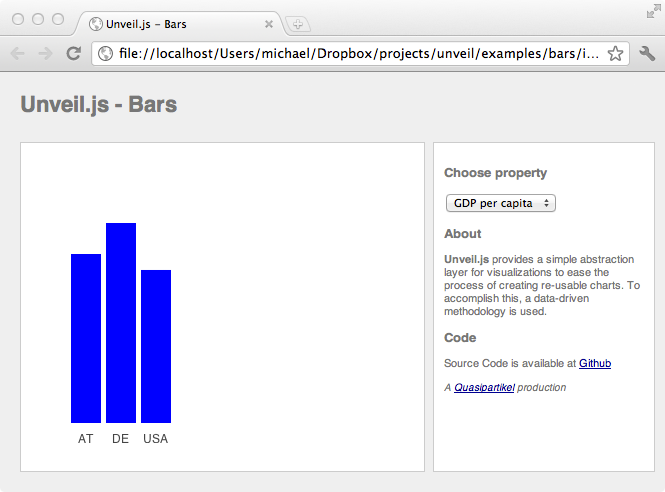
\includegraphics[width=1\textwidth]{bars}
\caption{A data-driven barchart generated from domain data expressed as a \texttt{Data.Collection}}
\label{fig:bars}
\end{figure}

\SuperPar Furthermore, a Scene object is created complete with a specified output display:

\begin{verbatim}
var scene = new uv.Scene({
  displays: [{
    container: 'canvas',
    width: 300,
    height: 300
  }]
});
\end{verbatim}

\SuperPar In order to guarantee that the bars fit on the available screen space, they need to be normalized accordingly. The function shown below maps values from an input domain (real numbers) to an output range (pixels).

\begin{verbatim}
function y(val) {
  var dMax = countries.properties().get(property)
              .aggregate(Data.Aggregators.MAX),
      oMax = 200;
  return parseInt(val/dMax * oMax);
}
\end{verbatim}


\SuperPar The scene will be initialized by adding a bar per data element in the collection. The height property encodes the value of the property under investigation.

\begin{verbatim}  
countries.items().each(function(c, key, index) {
  scene.add({
    id: "country_"+key,
    type: 'rect',
    x: 50+35*index,
    y: 280,
    width: 30,
    height: -parseInt(y(c.get(property)), 10),
    fillStyle: function() {
      return this.active ? 'orange' : 'blue'; 
    },
    interactive: true,
    actors: [
      {
        type: 'label',
        x: 15,
        y: 20,
        width: 30,
        height: 20,
        text: function() { return c._id.toUpperCase() },
        textAlign: 'center',
        fillStyle: '#444'
      }
    ]
  });
});
\end{verbatim}

\SuperPar Additionally, the visualization should allow dynamic switching between properties. For that purpose, property inspection features provided by Data.js are used to find out which numeric properties are available for the collection. By doing so, the visualization can be used with arbitrary collections, even if their structure differs.

\begin{verbatim}
countries.properties().each(function(p) {
  if (p.type === "number" && p.unique) {
    var option = $('<option value="'+p.key+'">'+p.name+'</option>');
    $('#property').append(option);
  }
});
\end{verbatim}

\SuperPar Every time the user selects a property, the bars need to be updated accordingly. In an event handler we are using the \texttt{animate()} method to specify an animated transition of the bar's height.

\begin{verbatim}
function update() {
  property = $('#property').val();
  countries.items().each(function(c, key, index) {
    scene.get("country_"+key).animate({
      height: -parseInt(y(c.get(property)), 10)
    }, 1.0);
  });
}
$('#property').change(update);
\end{verbatim}

\SuperPar Finally, the scene can be started.

\begin{verbatim}
scene.start();
\end{verbatim}


\section{Example Applications}
%%%-----------------------------------------------------------------------------


There is a range of examples available, that show different applications of Unveil.js. For each of them, the source code is available for inspection.

\subsection{Scatterplot}
%%%-----------------------------------------------------------------------------

\begin{figure}
\centering
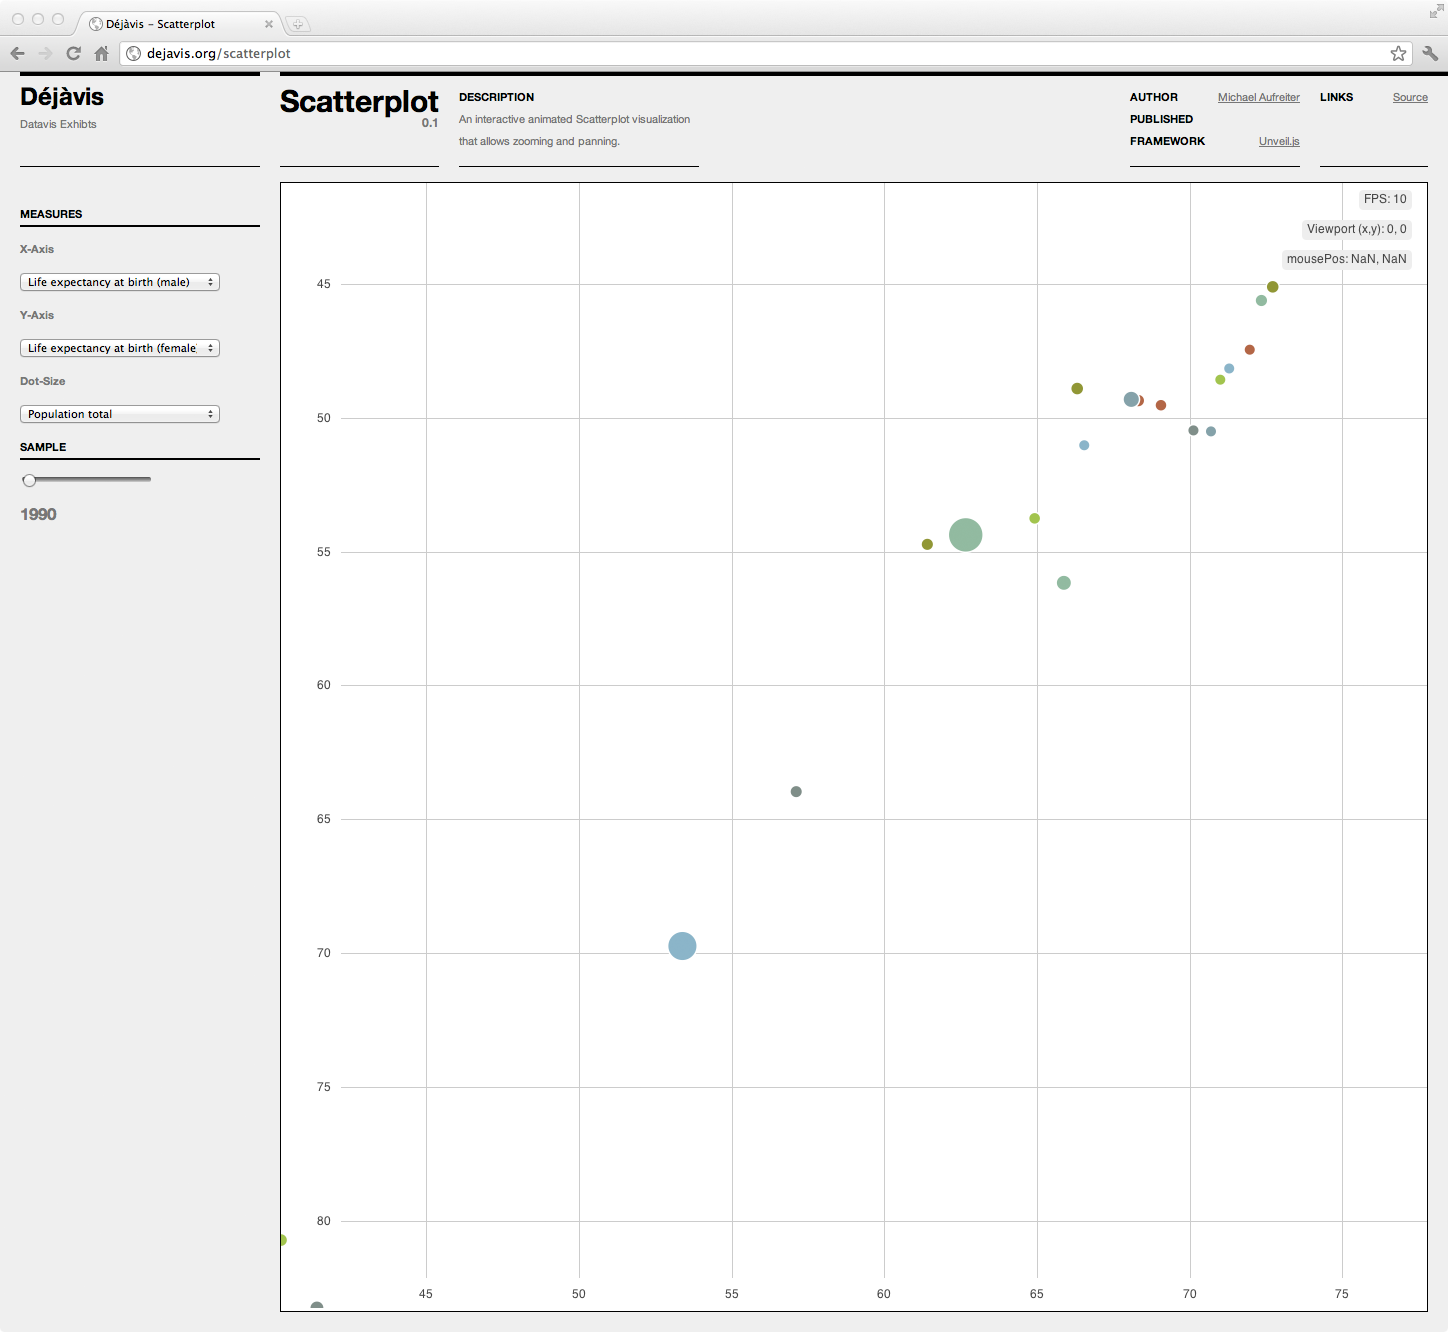
\includegraphics[width=1\textwidth]{scatterplot}
\caption{Scatterplot: A zoomable scatterplot visualization showing indicators for countries in three dimensions encoded using x-Axis, y-Axis and dot size.}
\label{fig:scatterplot}
\end{figure}

Scatterplot\footnote{http://github.com/michael/scatterplot}, as shown in Figure \ref{fig:scatterplot}, is an implementation of a zoomable scatterplot visualization that takes data in a uniform \texttt{Data.Collection} format. Users can assign different properties to certain axes. Each time they are changed, an animated transition takes place. Scatterplot makes intensive use of the data manipulation utilities provided by Data.js as well as matrix transformations for implementing zoom and pan behavior.


\subsection{Stacks}
%%%-----------------------------------------------------------------------------

Stacks\footnote{http://github.com/michael/stacks}, as shown in Figure \ref{fig:stacks}, is a visualization of categorical data. Musical Artists are displayed using self-organizing stacks that hold items of a certain group (e.g. genres like pop music, jazz, etc.). Based on meta-data, users can choose from ordinal properties that should be used to calculate group memberships. Transitions are animated accordingly. 

\begin{figure}
\centering
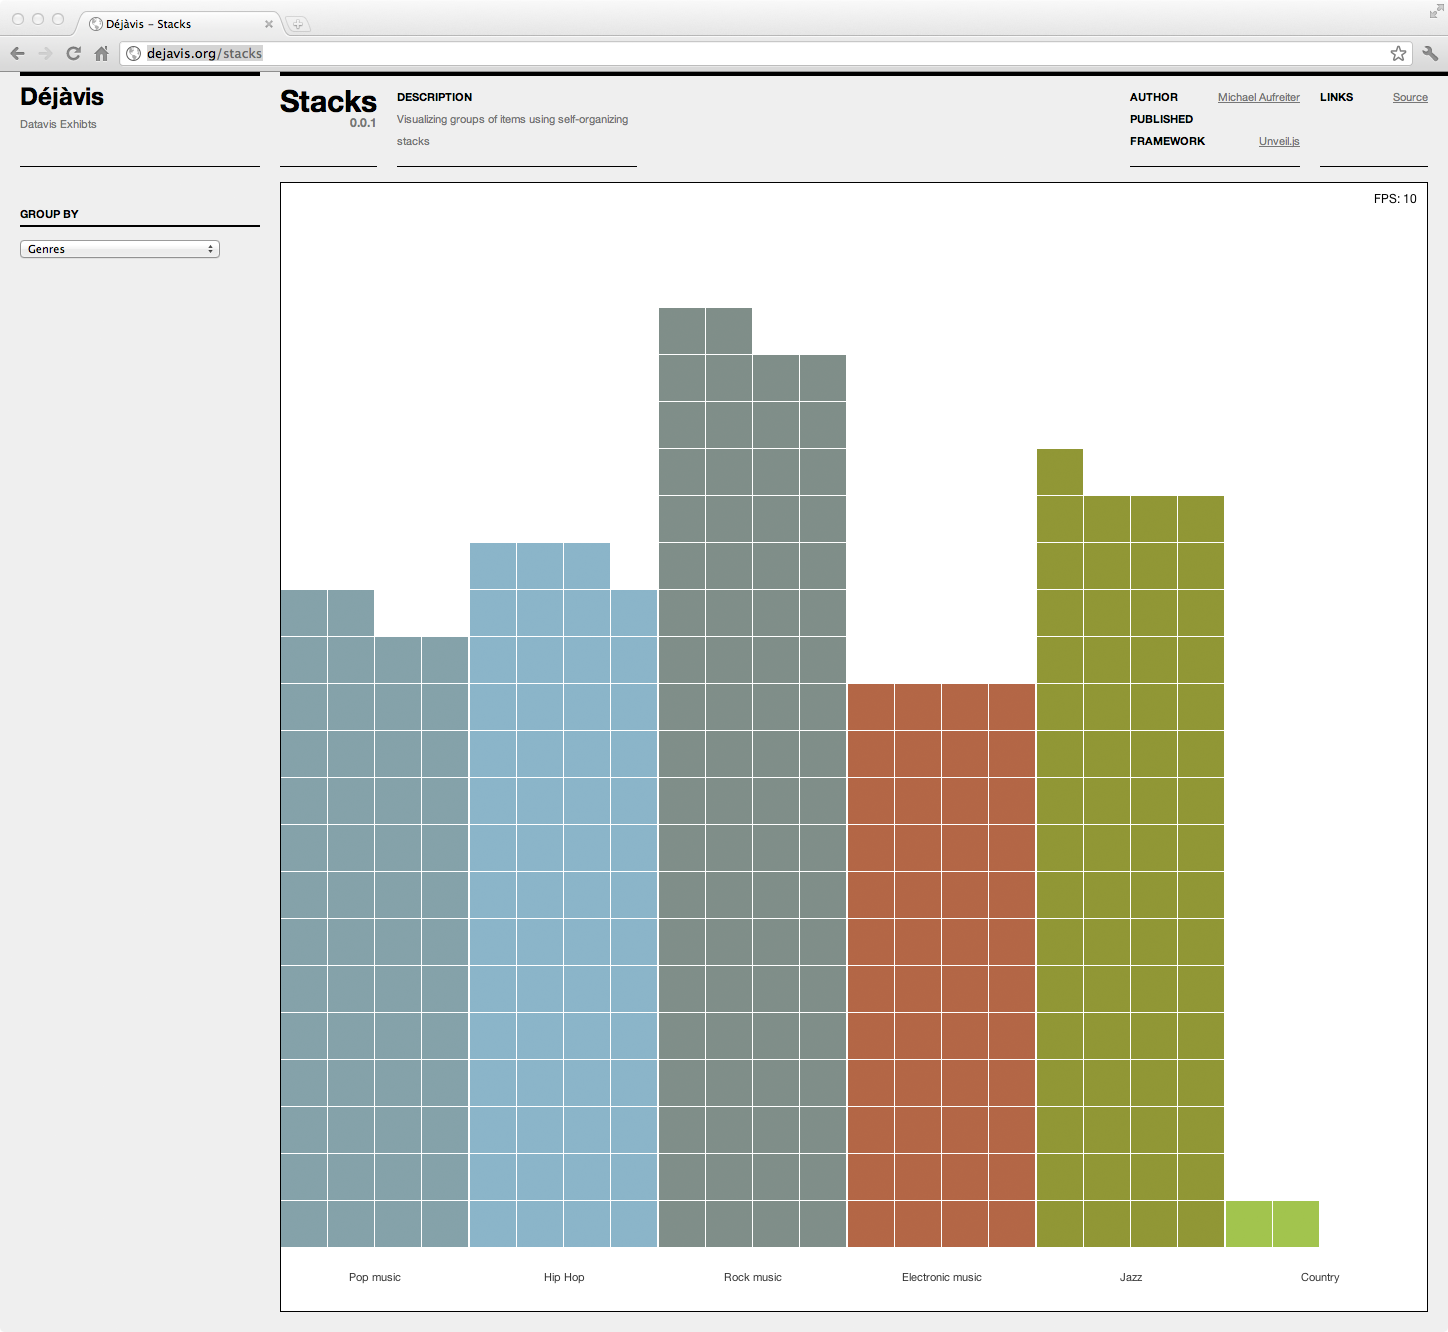
\includegraphics[width=1\textwidth]{stacks}
\caption{Self-organizing Stacks: Based on a layout algorithm groups and items are arranged on the screen.}
\label{fig:stacks}
\end{figure}

\end{english}